% !TEX root = ../Main.tex

\section{Differential Manifolds and Differentiable Maps}
\label{Section1}

\subsection{Review of General Topology}

Let $S$ be a set.

\begin{definition}
	A topology is a collection $\calT$ of subsets of $S$, called the open sets, such that:
	\begin{enumerate}[(i)]
		\item $\emptyset, S \in \calT$, where $\emptyset$ is the empty set.
		\item if $U_\alpha \in \calT$, for $\alpha\in A$, then $\bigcup_{\alpha\in A} U_\alpha \in \calT$
		\item if $U_1, \dots, U_n \in \calT$, $n \in \bbN$, then $\bigcap_{i=1}^n U_n \in \calT$  
	\end{enumerate}
\end{definition}

\begin{example}
	~
	\begin{enumerate}[(1)]
		\item $ S=\bbR^n$, $U \in \calT$ iff $U \subseteq S$ is open in the usual sense.
		\item If $(S, d)$ is a metric space, then it is a topological space.
	\end{enumerate}
\end{example}

\begin{definition}
	Let $(S,\calT)$ be a topological space. A basis for the topology of $S$ if the collection $B \subseteq \calT$ so that any $U\in\calT$ is the union of sets from $B$.
\end{definition}

\begin{example}
	~
	\begin{enumerate}[(1)]
		\item $\setst{B(x;\epsilon)}{ x \in \bbR^n, \epsilon\in\bbR^+}$ is a basis for the usual topology in $\bbR^n$.
		\item $\setst{B(x;\epsilon)}{ x \in \bbQ^n, \epsilon\in\bbQ^+}$ is a countable basis for $\bbR^n$.
	\end{enumerate}
\end{example}

\begin{definition}
	$(S,\calT)$ is second-countable if the topology $\calT$ has a countable basis.
\end{definition}

\begin{definition}
	$(S,\calT)$ is Hausdorff if for all $x,y \in S$, with $x\ne y$, there are open sets $U, V \subseteq S$ so that $x \in U$, $y\in V$ and $U\cap V=\emptyset$.
	\begin{figure}[H]
		\centering
		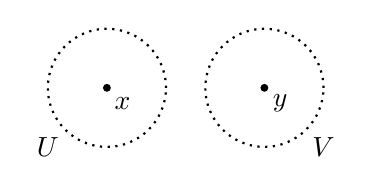
\begin{tikzpicture}
			\fill (0,0) circle(0.05) (2,0) circle(0.05);
			\draw[dotted, thick] (0,0) circle [radius=0.75] (0.2,-0.2) node {$x$} (-0.75,-0.75) node {$U$};
			\draw[dotted, thick] (2,0) circle [radius=0.75] (2.2,-0.2) node {$y$} (2.75,-0.75) node {$V$};
		\end{tikzpicture}
	\end{figure}
\end{definition}

The second-countability and ``Hausdorffness'' seams to be strange requirements but they are natural conditions, since the prototype of a manifold is the Euclidean space, which has these properties. If we do not impose these then many important results do not hold. For instance, we need Hausdorff condition in order to have unique convergence of sequences and uniqueness of ODE solutions.
Without second-countability, it is not certain that we can embed the manifold in a finite-dimensional Euclidean space.

Let's now define continuity in terms using topology language. Let $X, Y$ be any two topological spaces.

\begin{definition}	
	A map $f:X \to Y$ is continuous at $x\in X$ if for any open $V\subseteq Y$ containing $y$, there exists a open $U\subseteq X$ containing $x$ so that $f(U)\subseteq V$.

\begin{definition}
	A map $f:X\to Y$ is continuous if it is continuous al all $x\in X$.
\end{definition}

\begin{proposition}
	A map $f:X\to Y$ is continuous iff for all open $V\subseteq Y$, the preimage $f^{-1}(V) \equiv \setst{x \in X}{ f(x) \in V} \subseteq X$ is open in $X$.	
\end{proposition}

\begin{figure}[H]
	\centering
		\begin{tikzpicture}
			\begin{scope}[shift={(5,0)}]
				\draw plot [smooth cycle, tension=0.5] coordinates {(-2.4,-1)(-2.8,-0)(-3.2,0.5)(-3.2,1.3)(-2.7,1.7)(-1.7,1.5)(-1.2,0.5)(-0.7,-0.5)(-1.2,-1)};
				\draw[dotted,thick, fill=green, fill opacity=0.15] (-2,0) circle(0.55);
				\draw (-1.85,-0.15) node(x) {};
				%\fill (-2,0) circle(0.05);
				\node[below right = 0 and 0 of x] () {$V$};
				\node[above left = 1.1 and 0.4 of x] () {$Y$};
			\end{scope}
			\begin{scope}[shift={(-5,0)}]
				\draw plot [smooth cycle, tension=0.5] coordinates {(1.6,-1)(0.7,0)(0.6,0.5)(0.8,1.3)(1.3,1.7)(2.7,1.5)(3.1,0.5)(3.3,-0.2)(3.1,-1)};
				\draw[dotted, thick] (2.1,0) circle(1.0);
				\draw[dotted, thick, fill=green, fill opacity=0.15]  plot [smooth cycle, shift={(0.2,-0.1)}] coordinates {(1.84, -0.6)(1.48, -0.2)(1.44, 0.)(1.52, 0.32)(1.72, 0.48)(2.2, 0.4)(2.36, 0.)(2.48, -0.28)(2.4, -0.6)};
				\draw (2.15,-0.15) node(y) {};
				%\fill (2,0) circle(0.05);
				\node[above= 0.25 of y] () {$f^{-1}(V)$};
				\node[above left= 1.2 and 0.4 of y] () {$X$};
				\node[below right= 0.3 and 0.4 of y]  () {$U$};
			\end{scope}
			\node[anchor=north] at (-1.75, 0.65) (U) {};
			\node[anchor=north] at (1.70, 0.65) (fU) {};
			\draw[->,>=latex] (U) to [bend right=-30] node[above] {$f$} (fU);
		\end{tikzpicture}
		\caption{\color{red} Add caption to this figure}
\end{figure} 
\end{definition}

\begin{definition}
	A set $F\subseteq X$ is closed if $X\backslash F \subseteq X$ is open.
\end{definition}

\begin{proposition}
	A map $f:X\to Y$ is continuous iff $f^{-1}(F) \subseteq X$ is closed in $X$, for every closed $F\subseteq Y$ in $Y$.
\end{proposition}

\begin{definition}
	A continuous map $f:X\to Y$ is called a homeomorphism iff it has a continuous inverse $g:Y\to X$, such that $f \circ g = \mathrm{id}_Y$ and $g \circ f = \mathrm{id}_X$. We say that $X$ and $Y$ are homeomorphic. We write $g=f^{-1}$ and $X \cong Y$. 
\end{definition}

\subsection{Differential Manifolds}

\begin{definition}
	A topological manifold of dimension $m$ is a second countable, Hausdorff topological space $M$, so that any $p \in M$ has a open neighborhood $x \ni U \subseteq M$, which is homeomorphic with $\bbR^m$. For convenience, we will sometimes write $M^m\equiv M$ such that $\dim(M)=m$.
\end{definition}

\begin{remark}
	We might as well have said homeomorphic with an open subset of $\bbR^m$, because $B(0,\epsilon) = \setst{x\in \bbR^m}{ \norm{x} < \epsilon }$. To see that we can use the function
	\begin{align*}
		f:~&B(0,\epsilon) \to \bbR^m \\
		& x \mapsto \frac{x}{\epsilon-\norm{x}}
	\end{align*}
\end{remark}

\begin{remark}
	The \emph{Theorem of Invariance of Domain} states that if exists $\phi:\bbR^m \homeoto \bbR^n$, then $m=n$. Hence the definition is consistent.
\end{remark}

\begin{definition}
	A chart on a topological manifold $M^m$ is a tuple $(U,\phi)$, where $U\subseteq M$ is a open subset in $M$ and $\phi$ is a homeomorphism from $U$ to $V=\phi(U)\subseteq \bbR^m$ open in $\bbR^m$. If $0\in V$, we say that the chart is centered on $p$ if $\phi(0)=p$.

	\begin{itemize}
		\item $(U,\phi)$ is sometimes referred to as a coordinate patch.
		\item $(x_1(p),\dots,x_m(p))=\phi(p)$ are called local coordinates of the point $p$ in the chart $(U, \phi)$.
		\item $\phi^{-1}$ is also a homeomorphism and it is called a parametrisation.
	\end{itemize}

\end{definition}

We now are going to define the differential structure of the manifold.

\begin{definition}
	A $\calC^0$-atlas for $M$ is a collection $\calA = \setst{(U_\alpha, \phi_\alpha)}{\alpha\in A}$ of charts so that $\bigcup_{\alpha\in A} U_\alpha = M$.
\end{definition}

\begin{definition}
	A $\calC^k$-atlas for $M$ is a $\calC^0$-atlas such that
	\begin{align*}
		\theta_{\beta\alpha} \equiv {\phi_\beta \circ ({\phi_\alpha}\rvert_{U_{\alpha\beta}})^{-1}} \,:\, \phi_\alpha(U_{\alpha\beta}) \to \phi_\beta(U_{\alpha\beta}) ~,\quad
	\end{align*}
	are differentiable of class $\calC^k$ for all $\alpha,\beta \in A$, where $U_{\alpha\beta} \equiv U_\alpha \cap U_\beta$.
\end{definition}

\begin{remark}
	~
	\begin{itemize}
		\item The mappings $\theta_{\alpha\beta}$ are called transition maps (mathematics) or coordinate transformations (physics).
		\item Note that $U_{\alpha\beta}$ is open in $U_\alpha$ and $U_\beta$, so both $\phi_\alpha(U_{\alpha\beta})$ and $\phi_\beta(U_{\alpha\beta})$ are open in $\phi_\alpha(U_{\alpha})$ and $\phi_\alpha(U_{\alpha})$, respectively. Therefore $\phi_\alpha(U_{\alpha\beta})$ and $\phi_\beta(U_{\alpha\beta})$ are homeomorphic open sets in $\bbR^m$.
	\end{itemize} 
\end{remark}

\begin{figure}[H]
	\centering
	\centerline{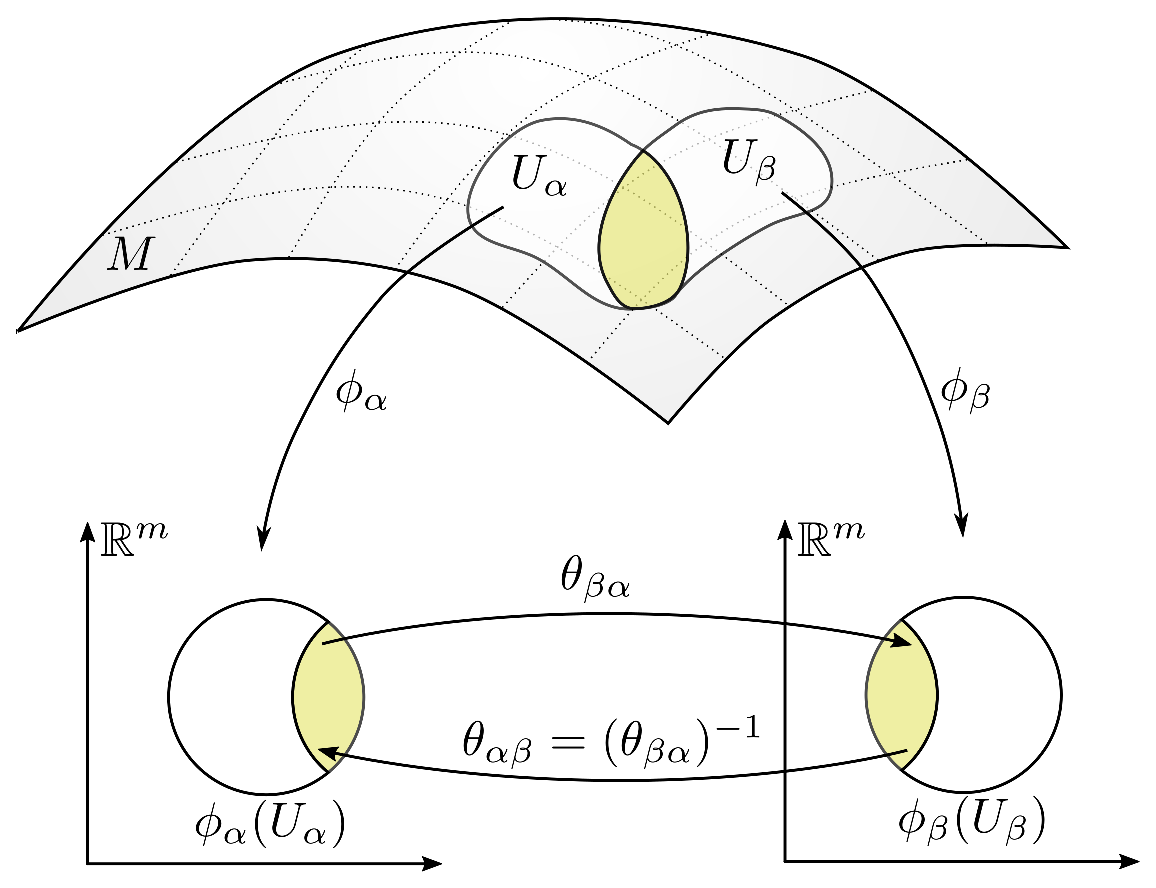
\includegraphics[width=0.7\textwidth]{Figures/diffhomeoreal.eps}}
	\caption{Figure describing homeomorphism between open sets in $M$ and in $\bbR^m$, with transition maps $\theta_{\alpha\beta}$.}
\end{figure}

\begin{definition}[Provisional]
	A differential manifold of class $\calC^k$ is a topological manifold $M$ together with a $\calC^k$ atlas.
\end{definition}

\begin{remark}[Smoothness]
	A smooth atlas is one where the transitions functions are of the class $\calC^\infty$, i.e. infinitely differentiable.
\end{remark}

\begin{example}
	~
	\begin{enumerate}[(1)]
		\item
		$M=\bbR^m$ is a differential manifold, with the trivial smooth $\calC^\infty$-atlas $\calA = \set{(\bbR^m, \mathrm{id})}$, where $\mathrm{id}(x)=x$. Note that $\bbR^m$ is open in $\bbR^m$.

		\item
		Let $M=S^{m}\equiv \setst{x\in\bbR^{m+1}}{\norm{x}=1}$. 
			
		We write $x=(x_0,x_1,\dots,x_m)$. The stereographic projections from $N=(1,0,\dots,0)$ and $S=(-1,0,\dots,0)$ are given from the following charts
		\begin{align*}
			\begin{split}
				\phi_N :~ &U_N \equiv S^m\backslash\set{N} \to R^m \\
				&(x_0, \dots, x_m) \mapsto \frac{1}{1-x_0}(x_1, \dots, x_m) 
			\end{split}
			~~
			\begin{split}
				\phi_S :~ &U_S \equiv S^m\backslash\set{S} \to R^m \\
				&(x_0, \dots, x_m) \mapsto \frac{1}{1+x_0}(x_1, \dots, x_m) 
			\end{split}
		\end{align*}

		\begin{figure}[H]
			\centering
			
\includegraphics[scale=0.3]{Figures/underconstruction.jpg}
			\caption{\color{red} Insert figure about describing the stereographic projection}
		\end{figure}
		
		\begin{fact}
			$\norm{\phi_N(p)} \,\norm{\phi_S(p)} =1$, for all $p\in U_N \cap U_S$.
			
			$\displaystyle \implies \theta_{NS}(y) = {\phi_N \circ ({\phi_S}\rvert_{U_{NS}})^{-1}}(y) = 
			\frac{(y_1,\dots,y_m)}{(y_1)^2+\dots+(y_m)^2} = \frac{1}{\norm{y}^2}\, y$

			Since this transition map is a map\footnotemark{} from $\bbR^m\backslash\set{0}$ to $\bbR^m\backslash\set{0}$ of class $C^\infty$, then $S^m$ is a smooth m-dimensional manifold.
			\footnotetext{This is called the inversion map and is actually one-to-one in the $m$-dimensional punctured Euclidean space $\bbR^m\backslash\set{0}$. It maps the region $0<\norm{y}<1$ to the region $\norm{y}>1$ and vice-versa, while leaving the unit sphere unchanged.}
		\end{fact}

		\begin{notabene}
			The topology on $S^m$ is the subspace topology, i.e. $U \subset S^m$ is defined to be open if it is of the form $U=S^m \cap V$ for some open $V\subseteq \bbR^m$.
		\end{notabene}
	
	\end{enumerate}
\end{example}

\begin{definition}
	Two charts $(\phi_\alpha, U_\alpha)$ and $(\phi_\beta, U_\beta)$ are said to be $\calC^k$-compatible if $\theta_{\beta\alpha} \equiv {\phi_\beta \circ ({\phi_\alpha}\rvert_{U_{\alpha\beta}})^{-1}}$ and $\theta_{\alpha\beta} = (\theta_{\beta\alpha})^{-1}$ are differentiable of class $\calC^k$. Note if $U\cap V = \emptyset$, we still say the transition map is smooth.
\end{definition}

\begin{definition}
	A $\calC^k$-atlas is maximal if it contains all $\calC^k$-compatible charts.
\end{definition}

% \begin{remark}
% 	In general there is not a unique maximal atlas on the manifold $M$. Consider $\bbR$ and the charts ($\bbR$, $\mathrm{id}$) and  ($\bbR$, $f$) , where $f(x)=x^3$. Each of these charts cover $\bbR$, but it's easy to check they are not smoothly compatible, so they generate distinct maximal atlases..3
% \end{remark}

\begin{lemma}
	Every $\calC^k$-atlas on a topological manifold is contained in a unique maximal $\calC^k$-atlas.
\end{lemma}

\begin{definition}
	A differentiable manifold of dimension $m$ and of class $\calC^k$ is topological manifold $M^m$ with a maximal $\calC^k$-atlas. This atlas is sometimes refer to as a differential structure.
\end{definition}

\begin{example}
	~
	\begin{enumerate}[(1)]
		\item
		If $M^m$ is a $\calC^k$-manifold of dimension $m$, then any open $U\subseteq M^m$ is also a $\calC^k$-manifold of dimension $m$.

		This is clear since for any open $U$ we can define charts
		$$\phi_\alpha\rvert_{U_\alpha\cap U} : U_\alpha\cap U \to \phi_\alpha(U_\alpha\cap U) \subseteq \bbR^m$$
		for any chart $\phi_\alpha : U_\alpha \to \phi_\alpha(U_\alpha) \subseteq \bbR^m$ on $M^m$.

		\item 
		If $U\subseteq \bbR^m$ is open and $g:U \to \bbR$ is of class $\calC^k$, then the graph of $g$
		$$ G = \setst{ (x,g(x)) }{ x \in U} \subseteq \bbR^{m+1} $$
		is also a $m$-dimensional manifold.
		
		Use the single chart $\phi : G \to U$, $(x, y) \mapsto x$, where $(x,y)\in U\times\bbR$. Note that $\phi^{-1}(x)=(x,g(x))$.

		\item \emph{Level hypersufaces} $f(p)=0$
		$$f:\bbR^{n+1}\to\bbR \qquad p=(x_1,\cdots,x_n,z)\mapsto f(p)$$
		If $\fracpd[z]{f}(p_0)\ne0$, for $p_0 \in f^{-1}(0) = \setst{p\in\bbR^{n+1}}{f(p)=0}$, then exists an open neighbourhood of $p_0$, $V\subseteq \bbR^{n+1}$, so that
		$$ f^{-1}(0) \cap V  = \setst{(x,g(x))}{ x \in U} \equiv U\times g(U) $$
		for a unique $\calC^k$-function $g:U\to\bbR$, for some open $U\subseteq\bbR^{n}$.
		Hence if $\nabla f (p)\ne 0 ~~\forall p \in f^{-1}(0)$, then $f^{-1}(0)$ will be a is a $\calC^k$-manifold of dimension $n$.
		
	\end{enumerate}
\end{example}

\subsection{Differential Maps}

\begin{definition}
	Let $U$ be open in $\bbR^n$. A function $f:U\to\bbR^m$ is differentiable at $x\in U$ if there is a linear map $D_x f : \bbR^n\to\bbR^m$ so that
	$$ f(x + h) - f(x) = D_x f(h) + o(h) ~~,$$
	where $\lim_{h\sto0} \frac{o(h)}{\norm{h}} = 0$. We may write  $D_x f(h)\equiv D_x f \cdot h$ to emphasize the linearity.
	
	A function $f:U\to\bbR^m$ is a differentiable iff it is differentiable in all $x\in U$.
\end{definition}

\begin{definition}
	Let $M^m$ be a smooth manifold.
	A function $f:M\to\bbR$ is differentiable at $p\in M$ if for some chart $(U,\phi)$, with $p\in U$, the function
	$$ f \circ\phi^{-1} : \phi(U) \subseteq \bbR^m \to \bbR$$
	is differentiable at $x=\phi(p)$.
\end{definition}

\begin{figure}[H]
	\centering
	
\includegraphics[scale=0.20]{Figures/underconstruction.jpg}
	\caption{\color{red} Insert figure about describing differentiability using charts}
\end{figure}

\begin{definition}
	A continuous function $f:M^m\to N^n$ is differentiable at $p\in M$ if for some chart $(U,\phi)$, the function
	$$ f \circ\phi^{-1} : \phi(U) \subseteq \bbR^m \to \bbR$$
	is differentiable at $x=\phi(p)$.
\end{definition}

\subsection{Inverse Function Theorem}

\subsection{Submanifolds and the Submersion Theorem}

\subsection{Compactness}

\subsection{Product and Quocient Manifolds}




\cleardoublepage